% !TEX root = Tesi.tex
\chead{}
\chapter{State of the art}

\section{Iot Devices : RFID, NFC, Beacons and Sensors}

The IoT can be used in a wide variety of fields: personal and health purposes, business and enterprise solutions, environmental applications just to list some. To achieve its goals, the Internet of Things ecosystem leverages a set of technologies to enable communication between devices and objects. Let's describe the most important ones :

\begin{itemize}
  \item \textbf{Radio Frequency Identification (RFID) } is a technology mostly used for one-way inventory tracking and supply chain applications. Products and boxes get marked using passive RFID tags containing logistics information readable from up until 100 meters distance by RFID readers providing them power. Specifically, each RFID tag comes with a small antenna and a silicon chip capable of storing the product information to facilitate the identification.  They are pretty small, and they can be efficiently combined with adhesive labels for cases and pallets, security cards, or implanted in pets, for example.  From an IT viewpoint, RFID readers (that can be handheld or mounted to a specific location such as a dock door) are responsible for reading and writing data from and to RFID tags transferring this data to backend IT systems.
  The primary difference with the most common electronic barcode mechanism is that barcode readers require “line-of-site”; the barcode reader must see the barcode lines to read the data and can only do that one barcode at a time while the RFID does not require it as tags can be scanned through a variety of materials.

  \item \textbf{Near Field Communication (NFC) } is a set of close-range wireless communication standards which offer functions similar to the most common Bluetooth and RFID technologies. Similarly to RFID, NFC can read special tags but unlike the first NFC tags can be used for virtually unlimited applications since the information can be easily retrieved from any conventional NFC-enabled device. Like Bluetooth, NFC supports two-way secure data exchange with a simple tap or wave among devices and it already comes with over 1 billion of them including an increasing number of tablets, PCs, household appliances, electronic devices, gaming consoles and of course smartphones. For a higher security and control, NFC only works within a close range of approximately 10 centimeters; this makes NFC perfect for more protected applications like payments or securely logging in at a location. 
 
  \item \textbf{Beacons} are small wireless devices that are capable of transmitting simple radio signals containing their identification number. Eventually, one of these signals gets detected by a nearby device such as smartphones using Bluetooth Low Energy technology. When this happens, the receiving device reads the beacon's ID, calculates the distance to the beacon and, depending on the result, triggers an action in a beacon compatible mobile app. Despite the simplistic concept Beacons are a substantial technological advancement; indeed they provide a way more precise tracking for indoor positioning and behavior compared with standard GPS technology. This simple communication, which is not heavy on power consumption, unfolds a wide range of new seamless interactions in a wide range of different areas. Retail, for example, is currently one of the most popular fields in which beacon technology is heavily used since it is offering an unprecedented way of tracking the in-store interaction between customers and retailers resulting in a more efficient set of personalized offers based on the acquired data. Other applications of the beacon technology, to mention a few, range from supporting and improving physical navigation in big spaces such as museums, airports and stadiums to helping impaired people on public vehicles.

  \vspace{0.5cm}
  \begin{figure}[htbp]
    \centering
      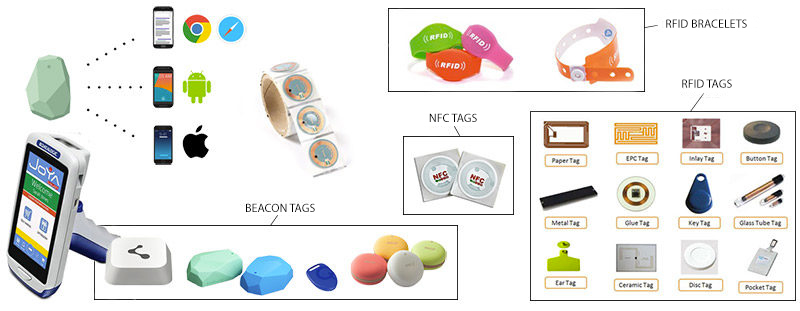
\includegraphics[height=6cm]{images/iot-devices.jpg}
    \caption{RFID, NFC and Beacon Tags}
    \label{fig:devices}
  \end{figure}
  \vspace{0.5cm}

  \item \textbf{Sensors} are the on-the-ground pieces hardware components of IoT doing the critical work of monitoring processes, taking measurements and collecting data. There exist hundreds of measurements that can be taken by sensors and they vary from temperature to proximity, from pressure to water quality, from gas detection to liquid level tracking. A variety of devices and solutions include these sensors while the general trend is moving towards multi-sensors platforms capable of incorporating different sensing elements at the same time. In the retail world, for example, they can make the store shelf "smarter" providing visibility from the product's arrival to final sale thanks to a combination of store shelf sensors, smart displays, digital price tags and high-resolution cameras. In fact, thanks to this technological ecosystem the retailer precisely knows what is on store shelves as well in stock rooms at any time effectively speeding up the restocking process. 
  Another example of an application would be around the next-generation of personalized self-tracking products in the form of wearables and smartwatches where a combination of accelerometers, GSR, temperature and heart rate sensors provide a comprehensive data insight on the activity of the user.   

  \vspace{0.5cm}
  \begin{figure}[htbp]
    \centering
      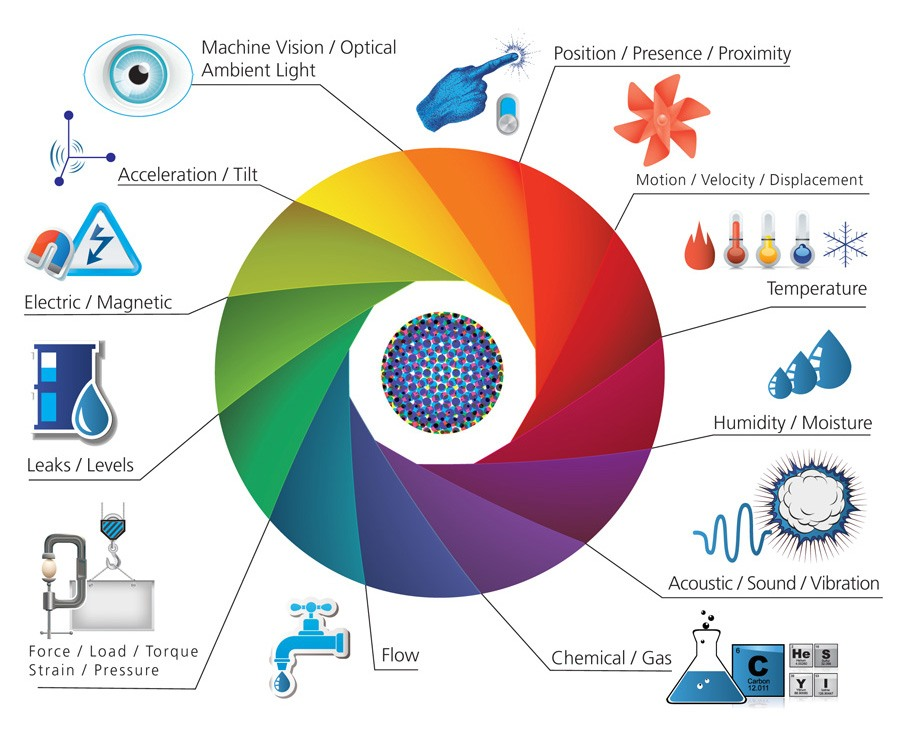
\includegraphics[height=10cm]{images/iot-sensors.jpg}
    \caption{Sensors ecosystem}
    \label{fig:sensors}
  \end{figure}
  \vspace{0.5cm}

\end{itemize} 

\section{Big Data and Predictive Analysis applications}

The concept of Big Data relates directly to the Internet of Things: IoT devices are indeed capable of collecting terabytes of data in a short amount of time, therefore being proficient a interpreting and analyzing such information is quite critical.

It's important to notice not only IoT devices are players capable of generating profiling data at such an incredibly high rate;  as per introduced in chapter \ref{section:data-web-mining} the modern Web represents another essential data source in this paradigm: social networks, for example, are capable of producing an endless stream of data describing user preferences and behaviors at any time.

This vast volume of data available to analyzers is behind the term Big Data which can be taught as a massive dataset, growing at a very high velocity in numerous formats from a variety of different origins.

To obtain business value from this amount of information, companies necessitate algorithms and solutions fitted to efficiently process, validate and give credibility to it, solutions beyond traditional systems currently used for managing and storing information, with high power and high calculation inclination that are efficient for sorting data in a structured and meaningful manner to detect relationships and patterns.

This new approach to data management differs from what companies used to do in the past when priorities were bound to an IT level governance only and they were solely accessed by a restricted set of users. 

It also becomes vital for a company to quickly and correctly identify new sources of big data when they become available on the market incorporating them into the data management platform following a constant continuous improvement logic.

It's quite hard to estimate in advance the added value brought by the Big Data analysis to the various application disciplines in which they can be applied, but they certainly warrant an improvement of the quality of the forecasts offering useful tools to take more prudent decisions supported by more robust empiric evidence.

In fact, Big Data analysis constitutes a fantastic instrument in the field of the decision-making throughout the whole organization pipeline minimizing the risks and reducing the errors caused by possibly wrong human intuitions at any level. For example, the Marketing department could potentially leverage big data for increasing marketing intelligence predicting customer interests while Logistics can utilize Big Data to better forecast product stock refurbishment or Operations can use it to optimize production requests.

\vspace{0.5cm}
\begin{figure}[htbp]
  \centering
    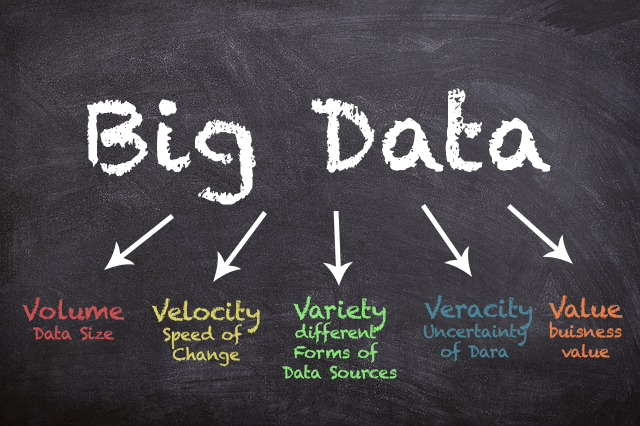
\includegraphics[height=8cm]{images/bigdata.png}
  \caption{The five fundamental Vs of big data }
  \label{fig:bigdata}
\end{figure}
\vspace{0.5cm}

In a nutshell, the potential applications mentioned above represent the core of the predictive analysis notion: the practice of extracting information from Big Data with the goal of determining patterns and predicting future outcomes and possible trends. 

It's important to notice that this kind of analysis does not offer a precise statement of what will happen in the future but rather they forecast what might occur with an acceptable level of reliability including what-if scenarios and risk assessment.

Focusing on the Marketing intelligence example mentioned above the benefits of using Predictive Analysis are immediate to understand. Indeed, it is one of the possible applications digital companies are embracing with the fastest rate nowadays, mostly because it allows them to offer better and more constructive experiences to the customers on every possible point of contact between the business itself and the clients with the goal of increasing customer loyalty and, naturally, incomes.


In detail, this process takes place using sophisticated algorithms and mathematical models on top of the big datasets of customers activity accessible from Big Data sources; eventually, this data gets sanitized, structured and filtered and finally grouped in a meaningful way. 

The behaviors and patterns of interaction detected by this process can indicate, for example, a more appealing product offer with a major chance of conversion for a particular customer profile segment.

\vspace{0.5cm}
\begin{figure}[htbp]
  \centering
    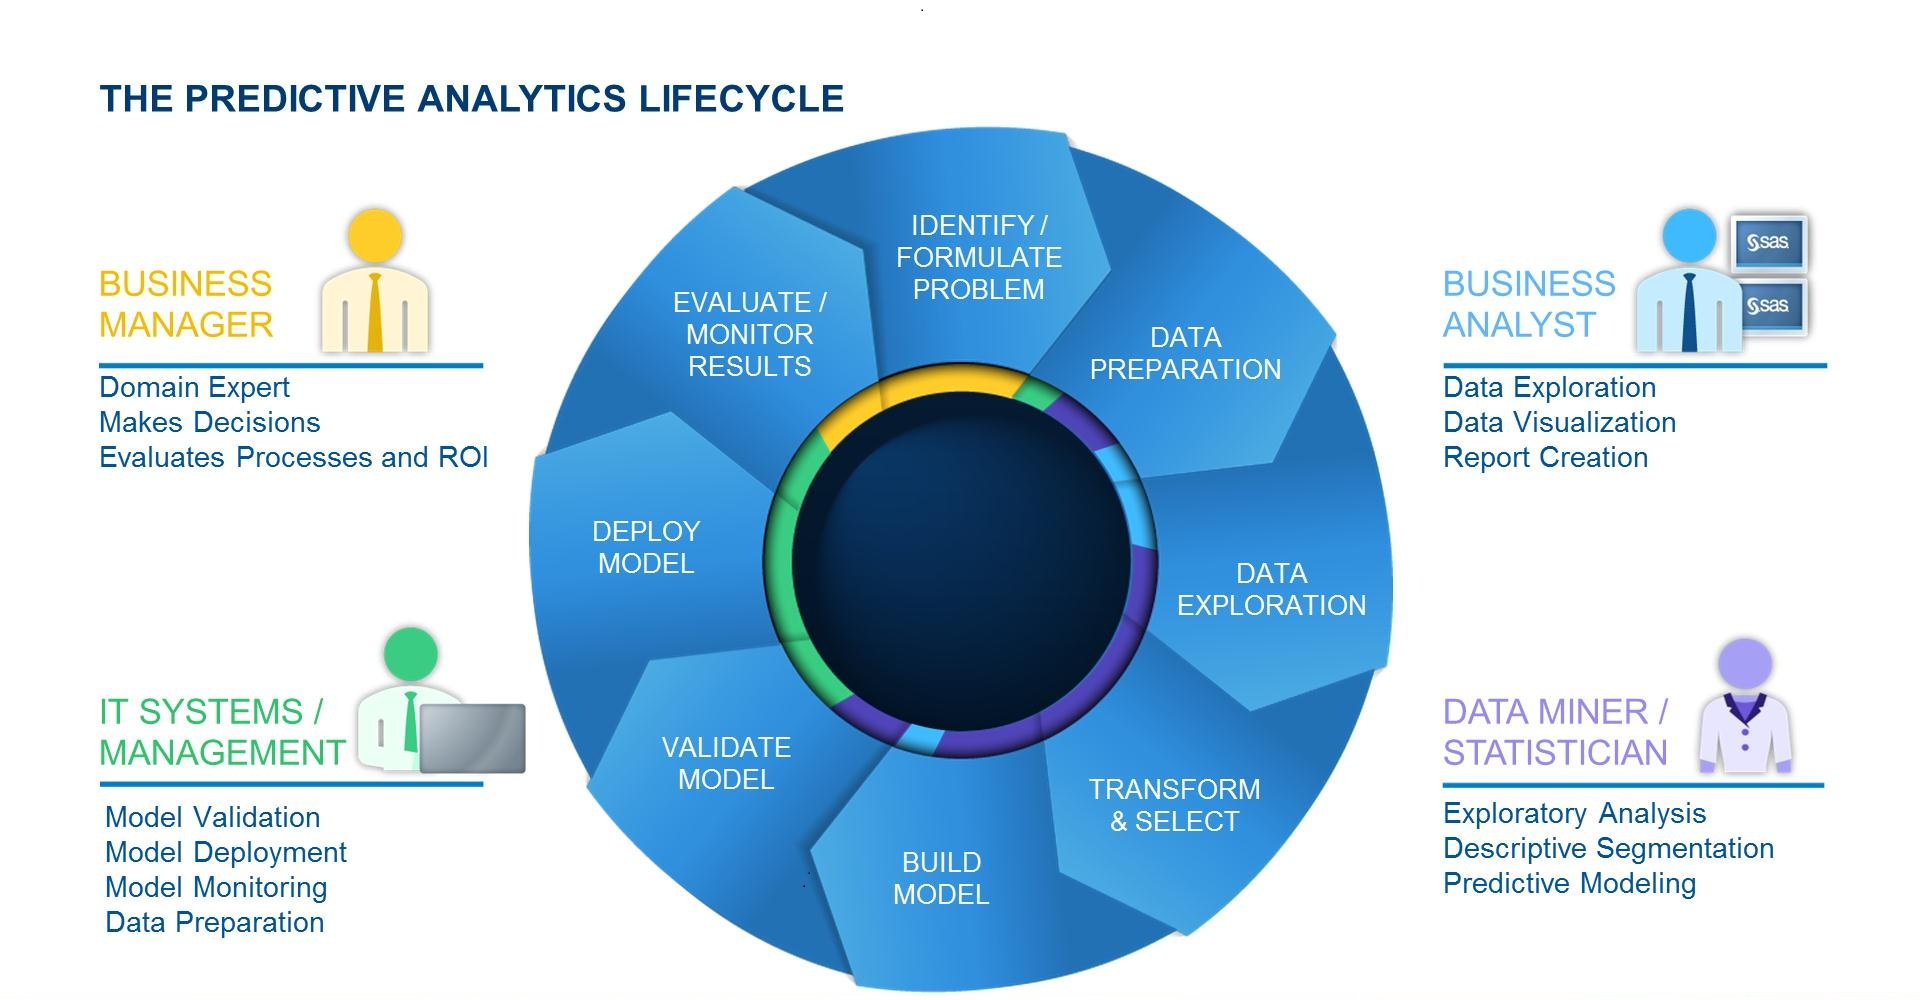
\includegraphics[height=8cm]{images/pa-lifecycle.jpg}
  \caption{The predictive analysis lifecycle }
  \label{fig:bigdata}
\end{figure}
\vspace{0.5cm}

As mentioned above different typologies and techniques are used to perform this type of analysis for behavioral prediction, these are the most important ones :



\begin{itemize}
    \item \textbf{Clustering or Unsupervised learning}:  This methodology groups similar individuals and identifies with high precision the enterprise's customer base. The algorithm processes hundred of attributes until it identifies the discriminating ones for a more efficient segmentation: the underlying idea is that several statistically significant groups behave in the same way. 

    The clusters obtained with this process are similar to groups determined through a priori segmentation; the fundamental difference between the two methodologies is that, while segmentation involves assigning customers to previously identified groups, clustering allows to distinguish the natural disposition of individuals in the different groups based solely on data and not preventive attributes definition. 

    Clusters can be of different types depending mostly on the criteria by which customers are grouped : product-based clusters, for example, gather all customers who tend to buy products or combinations of several products in the same category, brand-based clusters, on the other hand, focus on customers who prefer certain brands instead of others while behavior-based clusters combine consumers with similar buying behaviors, helping the marketing manager to identify the most appropriate way to address each of them.

    \item \textbf{Propensity models or Supervised learning}: This technique is based on probabilistic models using advanced machine learning techniques such as neural networks, logistic regression, random forest, and regression trees. The main purpose of these procedures is to predict future customer behavior based on past examples. Over time, these algorithms become more efficient, hardening forecasts with more data.

    \item \textbf{Reinforcement learning and Collaborative filtering}: This highly used technique in making predictions has major applications, one of the most famous one being the recommendation suggestion which offers tips on which products to buy. The recommendations are targeted and tailor-made for the client and they are obtained taking into consideration the entire relationship between customer and brand. Respectively they can upsell for higher value products, cross-sells to same category items or dynamically link other products based on the bought-together association.
  \end{itemize} 


 



%\addcontentsline{toc}{chapter}{}
